%%%%%%%%%%%%%%%%%%%%%%%%%%%%%%%%%%%
%%% Dynamic exposure studies
%%%%%%%%%%%%%%%%%%%%%%%%%%%%%%%%%%%

\section{Dynamic exposure \& health studies (1500 words)}
\label{sec:dynamicexposurehealth}

As has been discussed in the previous section, epidemiological studies investigating the relationship between health and air pollution generally fail to take account of places other than the subjects home address or area, they do not consider the effect of different micro-environments, and most do not attempt to examine the movement of the population. The epidemiological studies that are based upon these estimations may therefore be making incorrect conclusions. For example, \cite{Brauer2002} measured personal exposure compared to monitoring site exposure for PM$_{2.5}$ for 16 subjects in Canada and found that in 13 of the 16 subjects the measured ambient concentrations were under-representing exposure. Ashmore's review of literature focusing on children's exposure found that their exposure is closely related to concentrations in the home, at school, and in transport --- differing significantly from adults concentrations and general outdoor concentrations such as those at monitoring sites (\cite{Ashmore2009}). Although the links between health and air pollution are fairly clear as was discussed in section \ref{sec:healtheffects}, it might be that this miss-classification error is biasing calculated risk factors, regressions or coeffecients towards the null value (no association) i.e. once exposure classification is improved the relative risks of increases in exposure to pollutants may be greater than previously thought (\cite{Armstrong1990}).

This next section conducts a literature review of studies that consider these factors as part of an exposure study.




Keywords?
Activities of Daily Living, Adult, Air Pollution, Air Pollution, statistics \& numerical data, Environmental Monitoring, Environmental Monitoring, methods, Female, Geographic Information Systems, Humans, Inhalation Exposure, Inhalation Exposure, analysis, Inhalation Exposure, statistics \& numerical data, Male, Spain, Air Pollution, Air Pollution, analysis, Child, England, Environmental Exposure, Geographic Information Systems, Humans, Models, Reproducibility of Results, Sensitivity and Specificity, Software, Theoretical, Time Factors, Transportation

Need to be careful about what I bring in here. Carefully do a proper review. Start with some of the key recent papers such as de Nazelle and see what they reviewed/ their references. Maybe something like this from sciencedirect:

46 articles found for: pub-date > 2009 and "air pollution" AND "exposure" AND "urban" AND "pm2.5" AND "micro-environment"

Say that I'm interested in looking at studies that consider personal exposure and that contain information on time, place, use active sampling techniques, and were conducted after the year 2005 (random year chosen for example, will need to refine). Some sample text from another systematic review...

\begin{figure}[H]
\centering
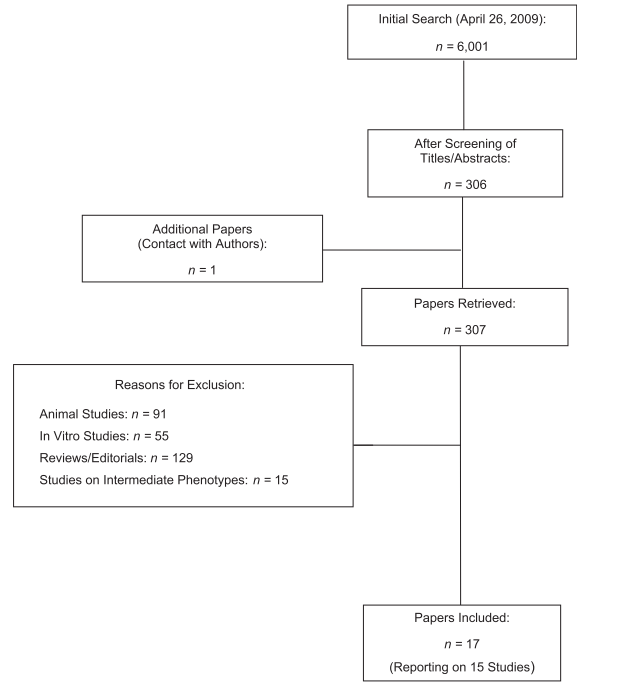
\includegraphics[scale=0.6]{systematic_review}
\caption{Inclusion and exclusion of papers for systematic review}
\label{fig:systematic_review}
\end{figure}

%%%%%%%%%%%%%%%%%%%%%%%%%%%%%%%%%%%
%%%% Activity diaries
%%%%%%%%%%%%%%%%%%%%%%%%%%%%%%%%%%%

\subsection{Activity diaries and the use of GPS (250 words)}
\label{subsec:avtivitydiaries}

\cite{DeNazelle2013}
GPS and accelerometers in mobile phones alongside surface models and activity diaries. Improving estimates of air pollution exposure through ubiquitous sensing technologies

\cite{Chaix2013} GPS tracking in neighborhood and health studies: a step forward for environmental exposure assessment, a step backward for causal inference?

\cite{Gerharz2013} -- Activity diary / gps / model / indoor outdoor. 

\cite{Kousa2002} --  A model for evaluation the poplation exposure to ambient air pollution in an urban area. Research that sought to predict long term exposure of population groups in urban areas by combining time activity data derived from the EXPOLIS study and modelled environmental NO2.

%%%%%%%%%%%%%%%%%%%%%%%%%%%%%%%%%%%
%%% Personal monitoring
%%%%%%%%%%%%%%%%%%%%%%%%%%%%%%%%%%%

\subsection{Personal monitoring (210 / 250)}
\label{subsec:personalmonitoring}

\cite{Kingham2013} used personal monitoring equipment and GPS devices to record individual’s exposure to traffic related pollutants of particulate matter and carbon monoxide on a number of routes in Christchurch, New Zealand. They compared the trip at the same time, day and route but by people travelling by bike (off-road) bike (on-road), car and bus during March 2009. Over 53 trips were completed. They found that cars had the highest mean CO exposure followed by bus, bike (on-road) and bike (off-road). For PM10 the pattern was similar but with much less variance. The highest was bus, followed by car, bike (on-road) and bike (off-road). PM$_{2.5}$ followed the same pattern. They concluded, at least in the city of their study, that car drivers are consistently exposed to the highest levels of carbon monoxide and ultrafine particles and that on-road cyclists are exposed to higher levels of CO PM$_{1}$ and UFP than off-road (back street) cyclists. Whether the results in this study could be generalised and applied to other cities, or even elsewhere in Christchurch, is unknown. The study did however benefit from very stable weather conditions (no rain, light wind) and Christchurch also has the advantage of suffering from little trans-boundary air pollution which could have confused the air pollution readings. Doing the same routes at the same time also improved the reliability of the study, as it meant that the results did not have to be adjusted for different background levels and/or increases in pollution from differing levels of transport at different times of the day.

\cite{Broich2011}
GPS, personal monitor, GRIMM 1.09 which does lots of PM fractions (but very heavy, needs back-pack?)

\cite{McCreanor2007}
Original oxford street study.

%%%%%%%%%%%%%%%%%%%%%%%%%%%%%%%%%%%
%%% Transport exposure
%%%%%%%%%%%%%%%%%%%%%%%%%%%%%%%%%%%

\subsection{Transport exposure (About 800 / 250)}
\label{subsec:transportexposure}

Aside from indoor air quality and air quality in specific outdoor locations such as street canyons detailed above, another subset of microenvironments to consider are vehicles and more generally, in-transport exposure. During the 2000’s a number of research groups started to look at how exposure varies between transport modes, and how the parameters of these transport modes can add further complications i.e. opening or closing windows on a car or where you sit on a bus. Whilst the variables to definitively understand someone’s in-vehicle exposure are almost too many to consider, it is important for us to at least try. By doing so it is hoped that ratios and formulas can be developed so that exposure scientists can model exposure during these times of a person’s day/week/month and attempt to quantify the effect that they have on health.

As can be seen from the data compiled by the Office for National Statistics in figure \ref{fig:transportprofiles}, the three most popular modes of transport in England and Wales over the last half a century have been car/van, followed by bus/coach and rail transport respectively. 

\begin{figure}[H]
\centering
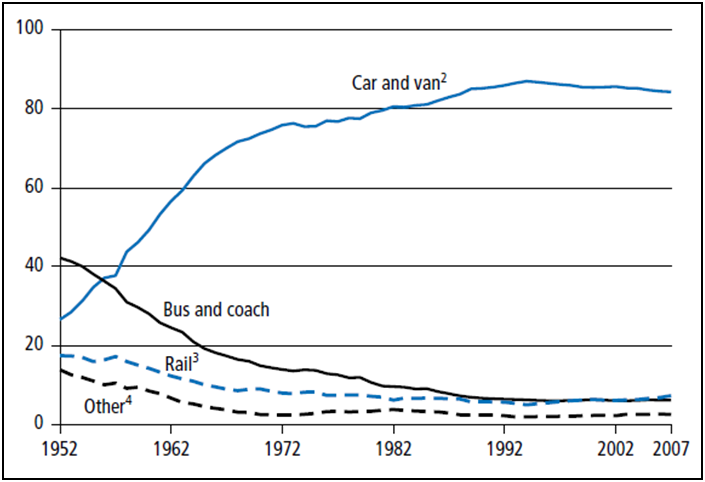
\includegraphics[scale=1]{transport_profiles}
\caption{Transport profiling from ONS census data}
\label{fig:transportprofiles}
\end{figure}

Whilst bus transport has clearly fallen in popularity across England and Wales over this time, this trend undoubtedly masks alot of intercity variation between cities. For example has bus transport declined at the same rate in London compared with Blackpool? Probably not. This isn’t an issue which I will consider any further at this time, other than to acknowledge it exists. The point is that a great number of people still frequently use the bus on a daily basis and that studies have found particle exposure in this environment to be higher than indoor locations and/or at urban monitoring sites.\medskip

\subsubsection{Bus exposure}
\label{subsubsec:busexposure}

To better understand this relationship (outdoor v. in bus) measurements were made simultaneously by placing an optical particle monitor in the middle of a bus in York over a period of three days in May 2007, and comparing the data recorded to measurements from an identical monitor on the bonnet of a car which followed the bus (\cite{Song2009}). Measurements / journeys were completed during the morning and evening rush hours and a total of 24 trips were completed. Figure \ref{fig:bus_ratios} shows how they found that the relationship between out-bus and in-bus concentrations was positively linear, with a higher gradient as particle size increases. Also that having the windows closed on the bus actually led to increased concentrations compared with having the windows open.

\begin{figure}[H]
\centering
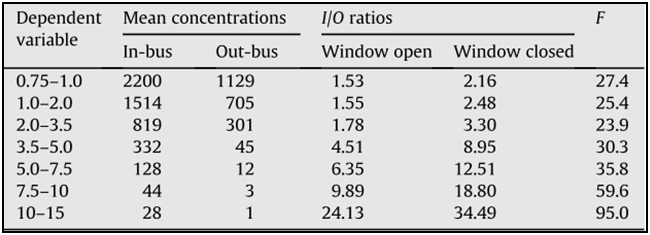
\includegraphics[scale=1.2]{bus_ratios}
\caption{Comparison of mean in-bus and out-bus particle concentrations}
\label{fig:bus_ratios}
\end{figure}

The authors of this study also propose that re-suspension of particles through passengers boarding and alighting has an important effect on particulate levels, but that this effect diminishes as particle size decreases.\medskip

Using data from this study the authors conclude by compiling a model for estimating the indoor/outdoor ratio of PM$_{0.75-10}$. The results of this ratio are in the range 3.76 – 7.66 depending on factors such as windows and passenger activity, and compare this ratio to other indoor/outdoor ratios in other studies to justify their findings (shown in Figure \ref{fig:summary_indoor_outdoor_bus}).

\begin{figure}[H]
\centering
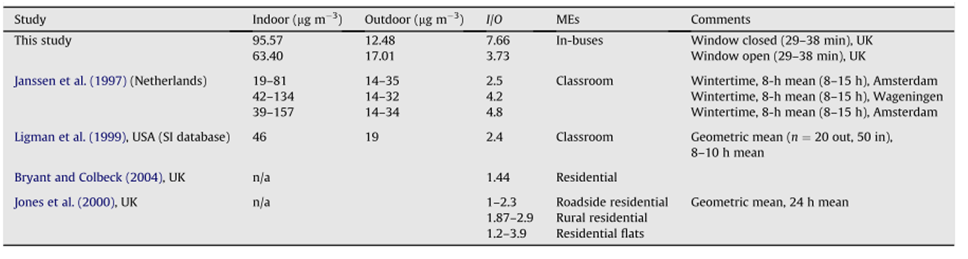
\includegraphics[scale=0.85]{summary_indoor_outdoor_bus}
\caption{Summary of indoor/outdoor bus ratios}
\label{fig:summary_indoor_outdoor_bus}
\end{figure}

However clearly the studies that are being compared to this are not like-for-like and only an indication of the exposure variance that might exist in this area. As the authors themselves acknowledge much more research needs to be done on this before, for example, generalised ratios for in-bus exposure can be developed. York is a relatively small town with relatively low ambient pollutant concentrations compared with the London, and the route that was studied was a park-and-ride system which was one-stop to one-stop and along a fast moving motorway from outside the town to the centre of a town. It would be interesting to see whether these ratios were similar in slow moving congested city centres such as London. The health implications of these ratios are also not discussed in this paper or others of it’s ilk (REF REF REF) as yet, however the development of exposure studies that take into account transport exposure such as this are a gradual step forward in this area. MAKE POINT THAT THEY DON’T TRY TO THINK ABOUT WHAT EFFECT THIS HAS ON A PERSONS DAILY / YEARLY EXPOSURE ETC. IT’S JUST NUMBERS OF PARTICLES REALLY. THIS IS A THEME OF THIS SECTION.\medskip

\subsubsection{Underground exposure}
\label{subsubsec:undergroundexposure}

In many worldwide cities the population travel between locations using metro systems. The London Underground was the first such system to open in 1863, but other cities have followed suite including New York, Paris, Seoul, Beijing, Berlin and Madrid. The size of each system varies in length, as does the power source, depth and speed of the trains, however the systems tend to be almost unanimously popular as a choice of travel mode for commuters (not surprising given that they were built for this purpose).  Air quality in these systems has not been extensively studied in many cities. Certainly not to the degree where general rules or ratios about the levels of exposure can be ascertained.\medskip

Table X summarises studies of the London Underground that took measurements of particulate matter. Do a short review of underground levels of exposure.

Good paper about underground exposure is \cite{Loxham2013}. Quite recent too. Ian did at Journal Club so I can use alot of his content. Bullets below.
point 1 - High concentrations of PM10, PM2.5 and PM0.1 observed in many underground railways. Sitzmann, B et al., Sci. Total Environ. 1999, 241 (1−3), 63−73. (London Underground). Bachoual, R et al., Chem. Res. Toxicol. 2007, 20 (10), 1426−1433. (Paris Metro). Ripanucci, G. et al., J. Occup. Environ. Hyg. 2006, 3 (1), 16−25. (Italian Rail tunnel).
point 2 - tend to give higher exposure that other methods of travel. Adams, H. S et al., Sci. Total Environ. 2001, 279 (1−3), 29−44.
Point 3 - Most PM thought to come from metals such as braking, tyre wear etc.
Point 4 - Found high content of Fe, which has been shown in many other studies.
Point 5 - Very different pollutant mix compared to traffic pollution on the street.
Point 6 - Though hard to compare this as the sampling site is not representative of London or many other cities actually. Alot of variation in this.

Another paper about underground. 'The London Underground: dust and hazards to health' (Seaton, A).
Point 1: They do some measuring on the tube. Cabins, platforms, stations.
Point 2: Find PM2.5 levels quite high, and then break this down into what it's made up of
Point 3: Say ~70\% is iron oxide, then some other metals make up another few percent (what's the rest?).
Point 4: Say that workers receive about 200mg/m3 over eight hours, which is way under UK occupational exposure for welding. So it's fine. What people are being exposed too isn't that toxic.

Another paper about underground is H.S. Adams. Fine particulate (PM2.5) personal exposure levels in transport microenvironments, London, UK. \cite{Adams2001}
1) 465 journeys and 61 volunteers, 3 weeks in the summer and 3 weeks in the winter
2) Three fixed routes at peak and off peak times of the day
3) Summer mean exposure was 34.5 for bicycle, 39 for for bus, 37.7 for car, and 247 for tube
4) Winter mean exposure was 23.5 for bicycle, 33.7 for bus, 38.9 for car, 157.3 for tube.
5) Significant variation between routes
6) Mean personal exposure levels in road transport were approximately double that of the concentration at an urban background fixed montior site.

Need to talk to Ian at this point. Is there something which goes against this? Better explanation/understanding required on my part as to why the above conclusions aren't satsifactor. Also I don't want to get caught up in toxicity. I want to talk about particle levels. Let the tox people sit between me and epi people...

%%%%%%%%%%%%%%%%%%%%%%%%%%%%%%%%%%%
%%% Indoor Exposure
%%%%%%%%%%%%%%%%%%%%%%%%%%%%%%%%%%%

\subsection{Indoor exposure (250)}
\label{subsec:indoorexposure}

In 2010 the World Health Organization published a report on indoor air quality (\cite{WorldHealthOrganization2010}) which tackles many of these key questions.\medskip

Indoor air pollution is estimated to cause approximately 2 million premature deaths mostly in developing countries. Almost half of these deaths are due to pneumonia in children under 5 years of age (\cite{WorldHealthOrganization2011})\medskip

Moelter, A, Lindley, S, de Vocht, F, Agius, R, Kerry, G, Johnson, K, Ashmore, M, Terry, A, Dimitroulopoulou, S \& Simpson, A 2012, 'Performance of a microenviromental model for estimating personal NO2 exposure in children' Atmospheric Environment, vol 51, pp. 225-233.\medskip

Although the effects of Write better intro to this. Good review of transport exposure here: Knibbs, L. D., Cole-Hunter, T., \& Morawska, L. (2011). A review of commuter exposure to ultrafine particles and its health effects. Atmospheric Environment, 45(16), 2611–2622. doi:10.1016/j.atmosenv.2011.02.065 . Aim is for health effects, but can take some of the findings and talk about levels and ratios

"Outdoor concentrations (mean, 42 fig/m3) exceeded indoor concentrations (mean, 35 jig/m3) but underestimated personal exposures (mean, 62 /ig/m3). The major part of the difference between personal and outdoor concentrations could be attributed to exposure to ETS, living along a busy road, and time spent in a vehicle. The results show a reasonably high correlation between personal and outdoor PM10 within individuals, providing support for the use of ambient PM10 concentrations as a measure of exposure in epidemiologic studies linking the day-to-day variation in partic- ulate matter air pollution to the day-to-day variation in health endpoints." from \cite{Janssen1998}.

%%%%%%%%%%%%%%%%%%%%%%%%%%%%%%%%%%%
%%% Dynamic Exposure
%%%%%%%%%%%%%%%%%%%%%%%%%%%%%%%%%%%

\subsection{Dynamic exposure (About 250 / 1000 words)}
\label{subsec:dynamicexposure}

As we have seen from the studies reviewed thus far, effectively and accurately quantifying human exposure to air pollution for epidemiological studies is fraught with problems. Studies that look at large numbers of people are difficult to accurately assign exposure values to as the people spend time in many different environments and are each exposed to different levels and types of pollution and different times. Indeed, even if assigning them accurate air quality data was possible, knowing where people spend their time is also difficult. \cite{Steinle2013} argue that the trend in this area of research is for the development of the personal monitoring approach, i.e. distribution of low-cost, accurate GPS devices combined with accurate low-cost unobtrusive portable air quality measurement devices (see section \ref{subsec:personalmonitoring} for further discussion of this area). A model of their theoretical approach is shown in \ref{fig:steinle_full_assessment}.

\begin{figure}[H]
\centering
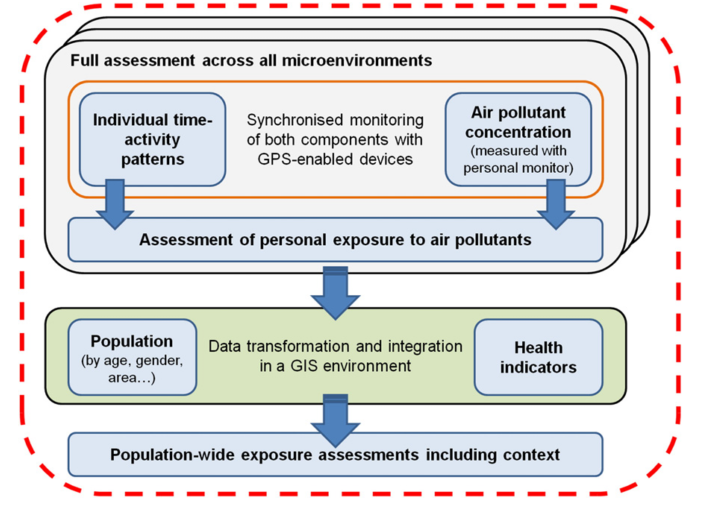
\includegraphics[scale=0.8]{steinle_full_assessment}
\caption{Conceptual model for the assessment of individual and population-wide exposure to air pollution including effects from \cite{Steinle2013}}
\label{fig:steinle_full_assessment}
\end{figure}

Unfortunately the technology for this type of study is not yet available, as the authors themselves note 'One limiting factor for the development of small, real-time mobile devices is the availability of low-power, high sensitivity sensors for priority air pollutants'.  I would add that even if such technology were in existance, then distribution and collecting the data on a large enough scale would also prove a stumbling block to this method.  Instead, modelling movements and air quality data, or a mix of the two approaches, seems a better approach. Particularly in the last five years researchers have started to do this.

%---------------------------------------
--NOW GO ON TO TALK ABOUT EVI DONS STUFF HERE.


\begin{figure}[H]
\centering
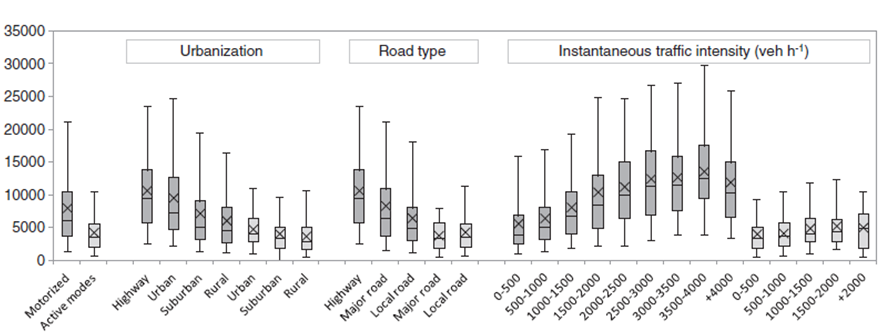
\includegraphics[scale=1]{road_type_exposure}
\caption{Not sure yet}
\label{fig:road_type_exposure}
\end{figure}

Number of people and amount of data was impressive.
Though temporal resolution of the microaeth was poor, and had some GPS problems.
“In urban areas exposure of motorists and active travelers is higher compared to exposure in more rural areas; the same holds for highways versus local roads for motorists.”

%-------------------------------------

In Milan during April 2005, Cattaneo et al found similar results in their research (\cite{Cattaneo2009}). They focused on ultrafine particles (=< PM10), using two hand-held Condensation Particle Counters (CPCs) to measure exposure when using different transport modes on a circuit of the town.

\begin{figure}[H]
\centering
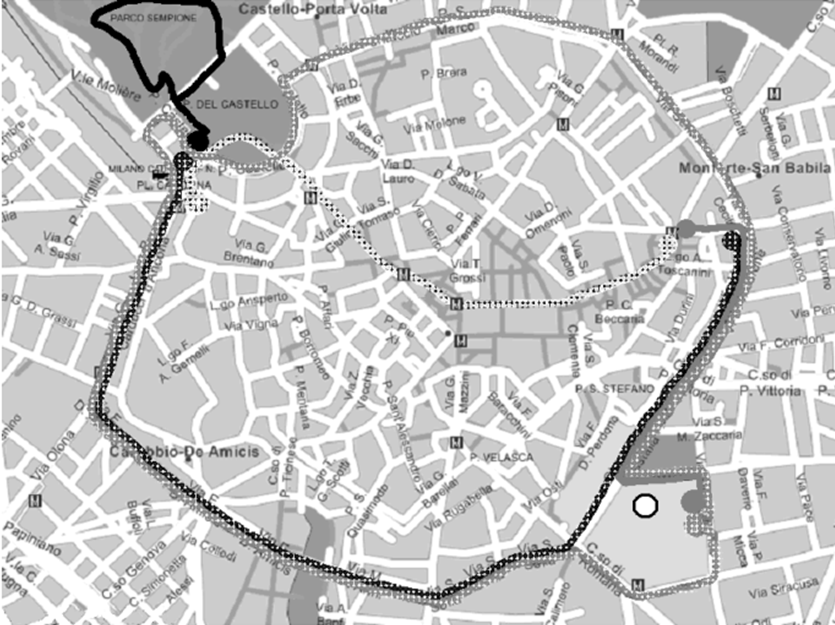
\includegraphics[scale=0.9]{monitoring_routes_used}
\caption{Monitoring route used by participants from \cite{Cattaneo2009}}
\label{fig:monitoring_routes_used}
\end{figure}

Song, WW, Ashmore, MR \& Terry, AC 2009, 'The influence of passenger activities on exposure to particles inside buses' Atmospheric Environment, vol 43, no. 39, pp. 6271-6278.

---Car versus. Bicycle
Int Panis, L., de Geus, B., Vandenbulcke, G., Willems, H., Degraeuwe, B., Bleux, N., … Meeusen, R. (2010). Exposure to particulate matter in traffic: A comparison of cyclists and car passengers. Atmospheric Environment, 44(19), 2263–2270. doi:10.1016/j.atmosenv.2010.04.028

---Car
(Dons et al. 2013)
From paper discussed earlier there is this graph which is worth talking about. Though wish it gave ratios instead of absolute values. Maybe I can make this point?

\begin{figure}[H]
\centering
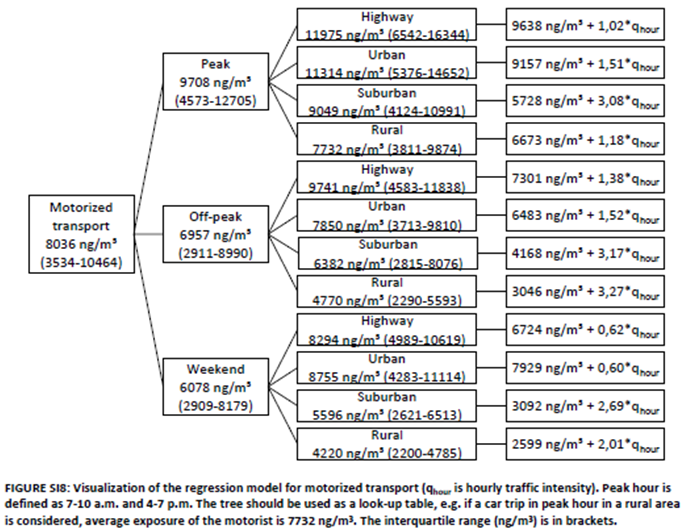
\includegraphics[scale=0.9]{transport_io_ratios}
\caption{Transport indoor/outdoor ratios from \cite{Dons2013}}
\label{fig:transport_io_ratios}
\end{figure}

\cite{DeNazelle2013}
-- 36 adults in Barcelona. Android app. GPS. Calfit. Larger batteries.
-- One week of data
-- Used modelled air pollution data on 5x5 grid
-- Inputted some missing GPS data
-- Interesting results
-- Bad - manual geocoding of key locations
-- Bad – Resolution of air pollution data

\begin{figure}[H]
\centering
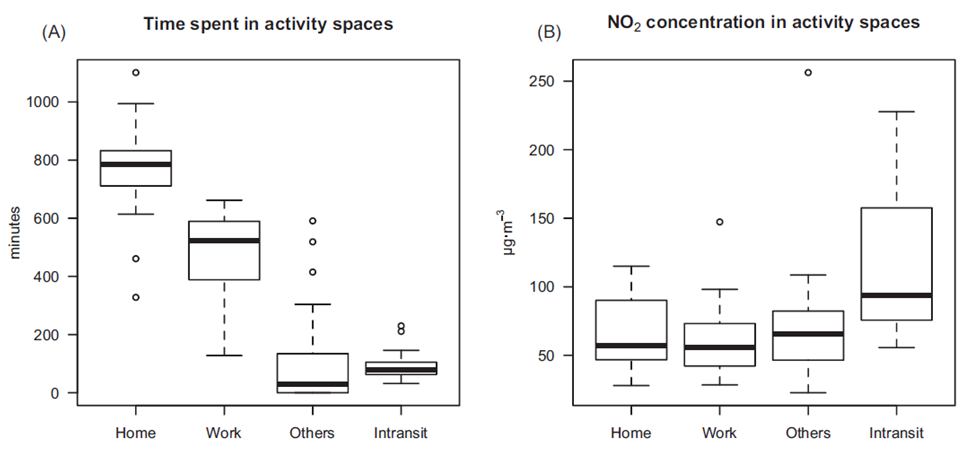
\includegraphics[scale=1]{time_no2_activity_spaces}
\caption{Time and NO2 in activity spaces from \cite{DeNazelle2013}}
\label{fig:time_no2_activity_spaces}
\end{figure}

\begin{figure}[H]
\centering
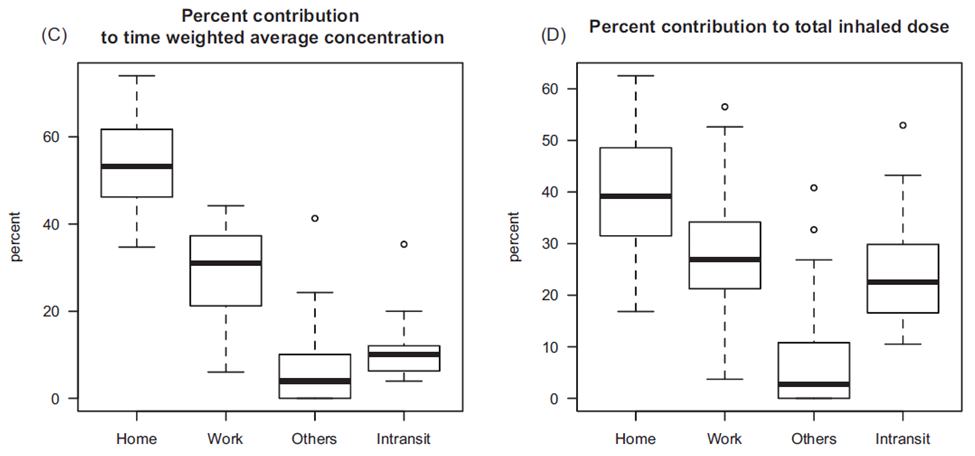
\includegraphics[scale=1]{time_dose_activity_spaces}
\caption{Time and dose in activity spaces from \cite{DeNazelle2013}}
\label{fig:time_dose_activity_spaces}
\end{figure}

\begin{figure}[H]
\centering
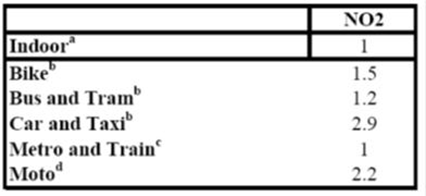
\includegraphics[scale=1]{nazelle_transport_ratios}
\caption{Transport ratios for the model from \cite{DeNazelle2013}}
\label{fig:nazelle_transport_ratios}
\end{figure}

\cite{Dhondt2012}
-- Looking at ‘static’ v. dynamic’ locations of people in Belgium
-- Considered NO2 and ozone
-- Agent-based model used for modelling behaviours and locations of people
-- Based on 8800 activity diaries
-- 5 million people modelled at 12km average resolution
-- Bad – Resolution of people poor
-- Bad – no microenvironment
-- Good – Well done for trying to do so many people at once
-- Good – One of the first to try a dynamic type approach
-- Good - Very good temporal resolution of air quality, but less so spatially.
-- Bad – No microenvironments attempted i.e. indoor? Vehicles?
-- Good – nice way of presenting the results however
-- “these findings confirm some of the results on the important role that commuting and human time-activity patterns have on population exposures to transport-related pollutants”

\begin{figure}[H]
\centering
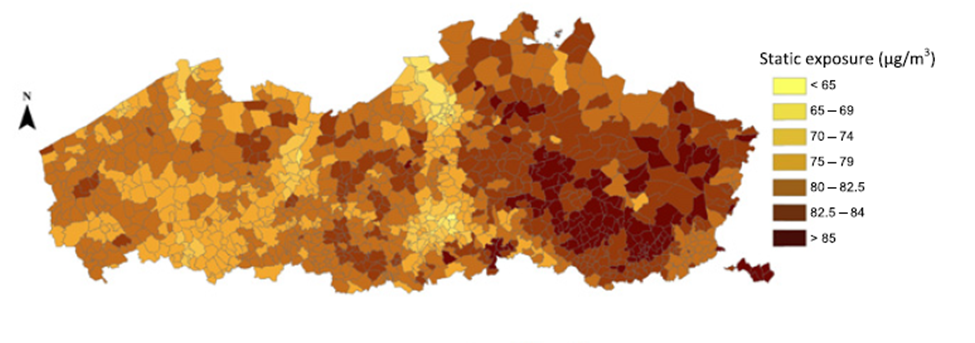
\includegraphics[scale=1]{dhondt_static_exposure}
\caption{Static exposure results from \cite{Dhondt2012}}
\label{fig:dhondt_static_exposure}
\end{figure}

\begin{figure}[H]
\centering
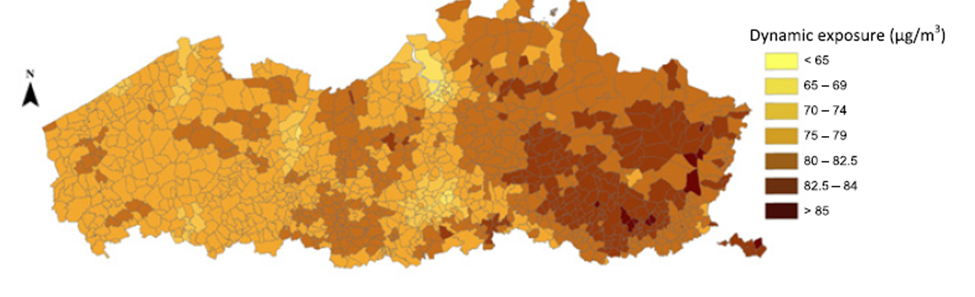
\includegraphics[scale=1]{dhondt_dynamic_exposure}
\caption{Static exposure results from \cite{DeNazelle2013}}
\label{fig:dhondt_dynamic_exposure}
\end{figure}

%%%%%%%%%%%%%%%%%%%%%%%%%
%%%% Summary of dynamic exposure
%%%%%%%%%%%%%%%%%%%%%%%%%
\subsection{Summary (0 / 100 words)}
\label{subsec:dynamicexposuresummary}

Finish the whole 'exposure miss-classification' section by summarising how these methods have been seeking to improve classification and that they have been able to do so by the use of smaller and more inexpensive monitoring equipment, better computers and software, more freely available data on people's location and habits. However problems remain about doing this on a large scale, validating it, and linking it to health outcomes robustly. But that very few studies have reached the panacea

\begin{figure}[H]
\centering
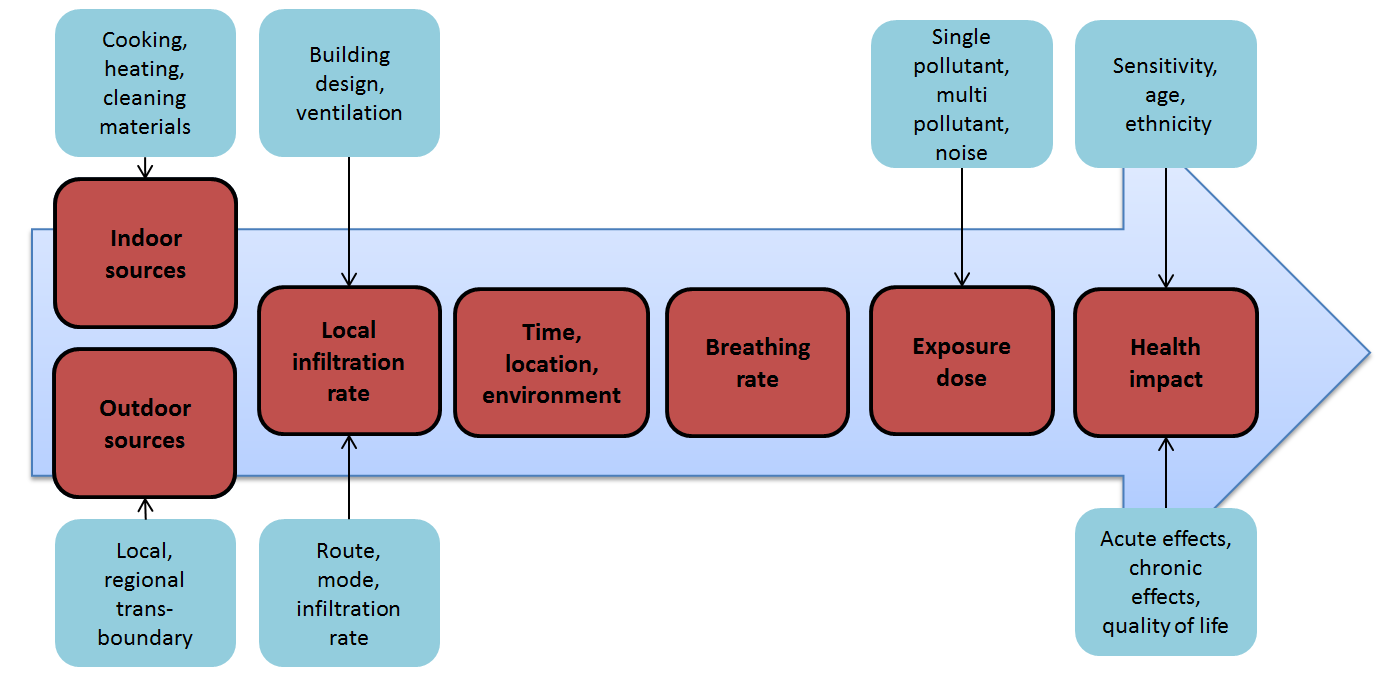
\includegraphics[scale=0.4]{james_exposure_diagram}
\caption{A conceptual dynamic exposure model}
\label{fig:james_exposure_diagram}
\end{figure}

Need a table in here. A summary of the literature. Spatial resolution, number of people, temporarl resolution, pollutants etc.

-- End with saying that most haven’t dealt with linking to health.